\begin{savequote}[75mm]
Basic research is what I am doing when I don't know what I am doing.
\qauthor{Wernher von Braun}
\end{savequote}

\chapter{$H\rightarrow WW^{*}\rightarrow \ell\nu\ell\nu$ Analysis Strategy}

\section{Introduction}

This chapter will present an overview of the strategy for searching for a Higgs boson in the 
\HWWfull decay topology. First, details of the signal final state and corresponding backgrounds are
presented. Then, the definitions of all of the objects used to reconstruct these final states 
are shown. Next, an overview of the variables used to reduce the backgrounds and enhance the
signal is given. Finally, the parameters of interest in the search and measurement will be defined, 
and a brief overview of the statistical treatment of the final Higgs candidates is given.


\section{Signal topology}

The analysis presented here and in subsequent chapters is the study of the Higgs boson in the $WW$ final state,
where each $W$ boson subsequently decays into a charged lepton and a neutrino. In its simplest form, the final state will then consist of two neutrinos and two charged leptons, each of which can be either an electron or a muon. If one or both of the $W$s decay to $\tau$ leptons, only leptonic decays of the $\tau$ are considered, leading to additional neutrinos in the final state but still giving two charged leptons as before. Neutrinos are not detected in ATLAS, so the final state ultimately consists of two reconstructed leptons and \met (denoted as $\MET$). Final states where both of the charged leptons are electrons or muons are referred to as the ``same flavor" final states, while those with one electron and one muon are referred to as ``different flavor".

\begin{figure}
  \vspace{20pt}
  \centering
  \hspace*{-32pt}
  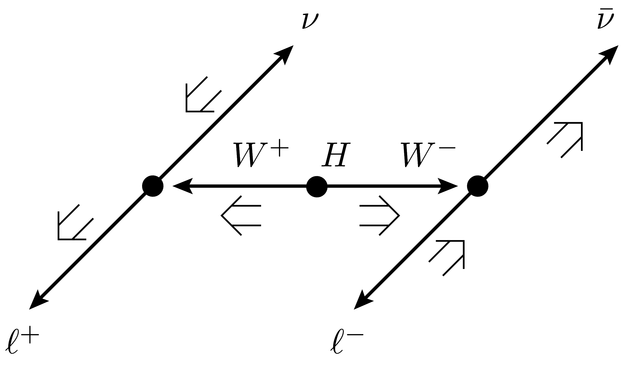
\includegraphics[width=0.42\textwidth]{figures/ww_spins}
  \caption{A cartoon of the WW final state. Momenta are represented with thin arrows, spins with thick arrows. \cite{WW2015}}
  \label{fig:WWdiagram}
\end{figure}


The final state leptons will also exhibit unique correlations due to the fact that they are arising from the decay of a spin zero resonance. In particular, the spins of the final state leptons and neutrinos must all cancel, as shown in figure~\ref{fig:WWdiagram}. Because the neutrino has a left handed
helicity and the anti-neutrino has a right handed helicity, the spin and momentum of the particles will be anti-aligned and aligned, respectively. In the transverse plane, the momenta of all four final state objects must cancel as well. With the constraint of having both the momenta and the spin alignments cancel, the final state kinematics strongly prefer having a small angle between the leptons in the transverse plane (low $\dphill$). This angular correlation will also lead to low values of the di-lepton invariant mass $\mll$. These unique signal final state kinematic correlations will be exploited to define the ultimate signal region. 

While the basic final state consists of two leptons and $\MET$, there can be additional objects as well depending on the production mode of the Higgs. As described in detail in Chapter 1, if the Higgs is produced via vector boson fusion production, there will be two additional forward jets in the event. Even in gluon fusion, one or more jets can be produced through initial state radiation from the incoming gluons. The analysis is separated into different signal regions depending on the number of hard jets reconstructed in the final state as well.


\section{Background processes}


\section{Object definitions}
\section{Isolating an $H\rightarrow WW^{*}\rightarrow \ell\nu\ell\nu$ signal}
\section{Background reduction in same-flavor final states}
\section{Parameters of interest and statistical treatment}